\documentclass{beamer}
\usepackage[utf8]{inputenc}
\usepackage{graphicx}
\usetheme{Antibes}
\title{Sentiment Analysis, News \& CAC40}
\author{Alexis Daboville}
\institute{Trinity College Dublin}
\date{\today}

\newcommand{\st}[0]{\superscript{st}}
\newcommand{\nd}[0]{\superscript{nd}}
\newcommand{\rd}[0]{\superscript{rd}}

\begin{document}
\begin{frame}
	\titlepage
\end{frame}

\begin{frame}{Introduction}
	\begin{itemize}
		\item Sentiment analysis
		\item News
		\item CAC40
	\end{itemize}
\end{frame}

\begin{frame}{Sentiments?}
	\begin{itemize}
		\item Opinions
		\item Subjectives
		\item Not facts
	\end{itemize}

	\pause

	Polarity:
	\begin{itemize}
		\item Positive: \emph{``This movie is {\color{green}great}.''}
		\item Negative: \emph{``This movie is {\color{red}bad}.''}
	\end{itemize}
\end{frame}

\begin{frame}{Sentiment Frequency}
	\begin{eqnarray*}
		words(day) &=& \textrm{A list of all words in the news of day}\\
  positive\_set &=& positive\_words\_set - economic\_words\_set\\
	positive\_words(day) &=& \sum_{w \in words(day)} \begin{cases}1 & \textrm{ if }w \in positive\_set\\ 0 & \mbox{ otherwise }\end{cases}\\
		positive\_freq(day) &=& \frac{length(positive\_words(day))}{length(words(day))}
	\end{eqnarray*}

	\pause

	Same method for negative sentiments.

\end{frame}

\begin{frame}{CAC40}
	\begin{itemize}
		\item Main French stock index
		\item Most important French companies
	\end{itemize}
\end{frame}

\begin{frame}{News Data: Problems}
	\begin{itemize}
		\item Data from several sources
		\item Paid archives
		\item \emph{Complex} systems to crawl
	\end{itemize}
\end{frame}

\begin{frame}{News Data: Solutions}
	\begin{itemize}
		\item Lexis Nexis
		\item Watir
	\end{itemize}
\end{frame}

\begin{frame}{News Data: Results}
	\begin{itemize}
		\item 500.000+ news
		\item From 9 economic newspapers/websites
		\item From January 1\st, 2004 to March 31\st, 2009
	\end{itemize}
\end{frame}

\begin{frame}{CAC40 Data}
	Downloaded from Yahoo! Finance
\end{frame}

\begin{frame}{Dictionaries}
	\begin{itemize}
		\item GI dictionary
		\item French translation by Stéphane Kazmierczak
		\item Stemming
		\item Economic dictionary
	\end{itemize}
\end{frame}

\begin{frame}
	\begin{figure}
		\caption{CAC40 close over time}
		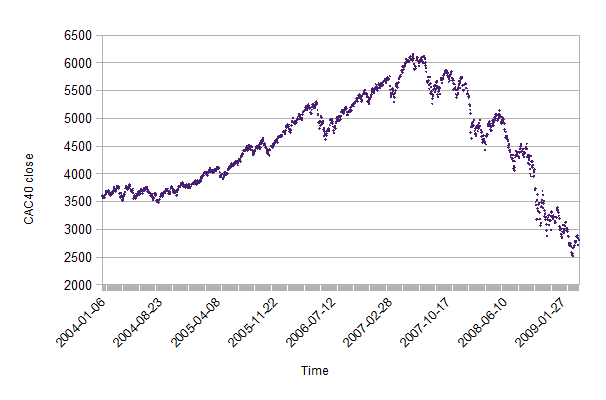
\includegraphics[scale=.5]{plots/time/cac.png}
	\end{figure}
\end{frame}

\begin{frame}
	\begin{figure}
		\caption{Positive sentiments frequency over time}
		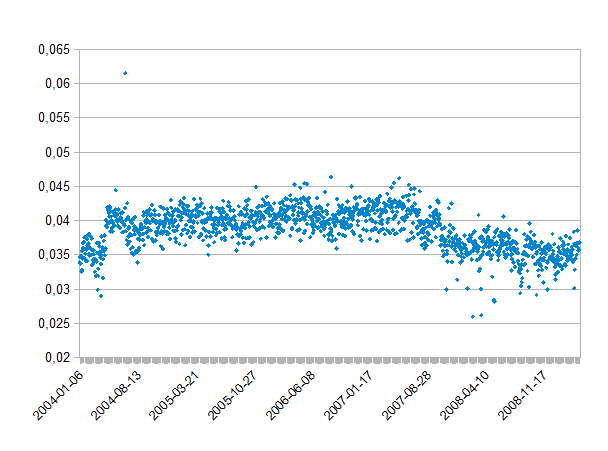
\includegraphics[scale=.5]{plots/time/pos.png}
	\end{figure}
\end{frame}

\begin{frame}
	\begin{figure}
		\caption{Negative sentiments frequency over time}
		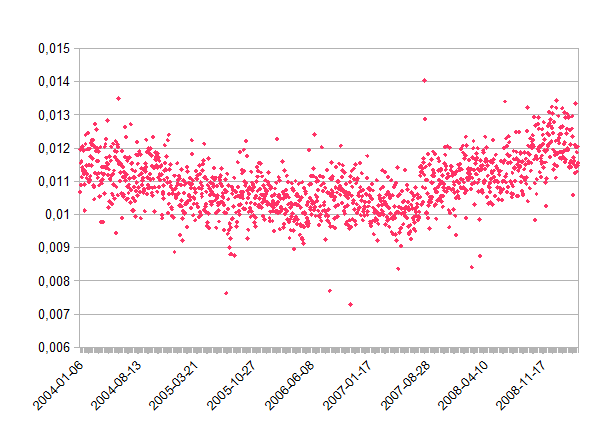
\includegraphics[scale=.5]{plots/time/neg.png}
	\end{figure}
\end{frame}

\begin{frame}
	\begin{figure}
		\caption{$\dfrac{positive\ sentiments\ frequency}{negative\ sentiments\ frequency}$ over time}
		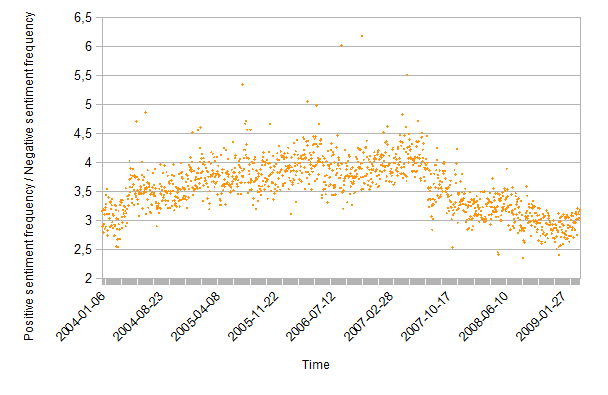
\includegraphics[scale=.5]{plots/time/posdivneg.png}
	\end{figure}
\end{frame}

\begin{frame}{Wrapping up}
	\begin{table}
		\scalebox{.75}{
			\begin{tabular}{|c | c | c | c|}
				\hline
				& Before mid-2007 & Mid-2007 & After mid-2007\\
				\hline
				CAC40 close & $\nearrow$ & $\rightarrow$ $\searrow$ & $\searrow$\\
				\hline
				Positive sentiments frequency & $\rightarrow$ & $\searrow$ & $\rightarrow$\\
				\hline
				Negative sentiments frequency & $\searrow$ & $\rightarrow$ & $\nearrow$\\
				\hline
				$\dfrac{Positive\ sentiments\ frequency}{Negative\ sentiments\ frequency}$ & $\nearrow$ $\rightarrow$ & $\searrow$ & $\searrow$\\
				\hline
			\end{tabular}
		}

		\caption{CAC40 and sentiments trends}
	\end{table}
\end{frame}

\begin{frame}{Return and Volatility}
	\begin{itemize}
		\item $return = \ln\frac{V_f}{V_i}$
		\pause \item Volatility: standard deviation of returns
	\end{itemize}
\end{frame}

\begin{frame}
	\begin{table}
		\scalebox{.75}{
			\begin{tabular}{|c || c | c | c|}
				\hline
				Sentiments date and CAC40 date & Positive sentiments & Negative sentiments & $\dfrac{Positive}{Negative}$\\
				\hline
				previous(day) and day & -0.0280 & -0.0583 & 0.0292\\
				\hline
				day and day & 0.0450 & -0.0764 & 0.0956\\
				\hline
				next(day) and day & 0.0491 & 0.0305 & 0.0089\\
				\hline
			\end{tabular}
		}

		\caption{Pearson correlation between sentiments returns and CAC40 returns.}
	\end{table}
\end{frame}

\begin{frame}
	\begin{table}
		\scalebox{.75}{
			\begin{tabular}{|c || c | c | c|}
				\hline
				Sentiments date and CAC40 date & Positive sentiments & Negative sentiments & $\dfrac{Positive}{Negative}$\\
				\hline
				previous(day) and day & -0.0655 & 0.0537 & -0.0899\\
				\hline
				day and day & -0.0201 & -0.0681 & 0.0433\\
				\hline
				next(day) and day & 0.0936 & 0.0473 & 0.0247\\
				\hline
			\end{tabular}
		}

		\caption{Pearson correlation between sentiments returns and CAC40 volume returns.}
	\end{table}
\end{frame}

\begin{frame}
	\begin{table}
		\begin{center}
			\begin{tabular}{|c | c | c|}
				\hline
				Positive sentiments & Negative sentiments & $\dfrac{Positive}{Negative}$\\
				\hline
				0.1240 & -0.1029 & -0.3180\\
				\hline
			\end{tabular}
		\end{center}

		\caption{Pearson correlation between sentiments volatility and CAC40 volatility (over 30 days).}
	\end{table}

	\begin{table}
		\begin{center}
			\begin{tabular}{|c | c | c|}
				\hline
				Positive sentiments & Negative sentiments & $\dfrac{Positive}{Negative}$\\
				\hline
				-0.2061 & 0.0846 & 0.0567\\
				\hline
			\end{tabular}
		\end{center}

		\caption{Pearson correlation between sentiments volatility and CAC40 volume volatility (over 30 days).}
	\end{table}
\end{frame}

\begin{frame}{Better hypothesis? I}
	Consecutive close are highly correlated
\end{frame}

\begin{frame}{Better hypothesis? II}
	$$cac40\_close(t) = \alpha_0 + \sum_{i = 1}^{n}\left(\alpha_i\times{}cac40\_close(t - i)\right) + \varepsilon(t)$$
\end{frame}

\begin{frame}{Better hypothesis? III}
	\begin{itemize}
		\item Autoregressive model (to find $\alpha_i$)
		\item Trained over 90\% of the data
		\item Used to predict the remaining 10\%
		\item Computed $\varepsilon(t)$ for each day
	\end{itemize}
\end{frame}

\begin{frame}
	\begin{table}
		\scalebox{.75}{
			\begin{tabular}{|c || c | c | c|}
				\hline
				Sentiments date and CAC40 date & Positive sentiments & Negative sentiments & $\dfrac{Positive}{Negative}$\\
				\hline
				previous(day) and day & -0.06 & 0.17 & -0.10\\
				\hline
				day and day & 0.17 & -0.05 & 0.17\\
				\hline
				next(day) and day & -0.08 & 0.27 & 0.17\\
				\hline
			\end{tabular}
		}

		\caption{Pearson correlation between sentiments and $\varepsilon(t)$}
	\end{table}
\end{frame}

\begin{frame}{Volume?}
	In fact we can apply the same hypothesis to CAC40 volume
\end{frame}


\begin{frame}
	\begin{table}
		\scalebox{.75}{
			\begin{tabular}{|c || c | c | c|}
				\hline
				Sentiments date and CAC40 date & Positive sentiments & Negative sentiments & $\dfrac{Positive}{Negative}$\\
				\hline
				previous(day) and day & -0.13 & 0.16 & -0.24\\
				\hline
				day and day & 0.13 & 0.30 & -0.16\\
				\hline
				next(day) and day & 0.05 & 0.14 & -0.09\\
				\hline
			\end{tabular}
		}

		\caption{Pearson correlation between sentiments and $\varepsilon_v(t)$}
	\end{table}
\end{frame}

\begin{frame}{Conclusion}
	\begin{itemize}
		\item Things learned
		\pause \item Results
		\pause \item Improvements
	\end{itemize}
\end{frame}

\begin{frame}
	Thanks for listening, questions?
\end{frame}
\end{document}

